\section{Buck converter}
\subsection{What is a buck converter?}
A \textit{buck converter}, also known as a \textit{step-down converter}, is a type of DC-DC converter that efficiently converts a higher input voltage to a lower output voltage. The buck converter operates on the principle of pulse width modulation (PWM), controlling the duty cycle of the switch to regulate the output voltage.

\subsubsection{Applications}
Buck converters find widespread use in various electronic systems where it is necessary to step down voltage levels. They are commonly employed in power supplies for electronic devices, battery chargers, and voltage regulation circuits. Additionally, buck converters are frequently utilized in applications requiring efficient power management, such as in electric vehicles, renewable energy systems, and portable electronic devices where efficiency is a key component.

\subsection{What is the difference between a buck converter and a voltage regulator?}
The main differences between a \textit{buck converter} and a \textit{voltage regulator} lie in their operating principles, efficiency, and applications.

\begin{enumerate}
  \item \textbf{Operating Principle:}
    \begin{itemize}
      \item \textbf{Buck Converter:} Operates by switching the input voltage on and off at a high frequency, regulating the output voltage by controlling the duty cycle of the switch.
      \item \textbf{Voltage Regulator:} Adjusts the output voltage by dissipating excess energy as heat. The regulation is achieved through the use of linear components.
    \end{itemize}
  \item \textbf{Efficiency:}
    \begin{itemize}
      \item \textbf{Buck Converter:} Generally more efficient than voltage regulators, especially in scenarios where there is a significant voltage difference between the input and output.
      \item \textbf{Voltage Regulator:} Can be less efficient, particularly when dropping voltage by a large margin, as the excess energy is dissipated as heat.
    \end{itemize}
  \item \textbf{Cooling Requirement:}
    \begin{itemize}
      \item \textbf{Buck Converter:} Generates less heat due to its switching nature, often requiring less or no additional cooling elements.
      \item \textbf{Voltage Regulator:} Produces heat that needs to be dissipated, often requiring additional cooling elements such as heat sinks.
    \end{itemize}
  \item \textbf{Suitability for High Voltage Differences:}
    \begin{itemize}
      \item \textbf{Buck Converter:} Well-suited for applications with higher voltage differences, providing efficient voltage reduction.
      \item \textbf{Voltage Regulator:} Less suitable for high voltage differences due to increased heat dissipation and lower efficiency.
    \end{itemize}
\end{enumerate}


\subsection{What does a buck converter do in our application?}
In our application, which involves designing an electric bike motor, a \textit{buck converter} is employed to efficiently reduce voltage levels. This is crucial for optimizing the overall efficiency of the system. Diego Zuidervliet\cite{zuidervliet2024} recommended the use of Webench from Texas Instruments, a power simulator that simulated the creation of three different circuits utilizing the same switching IC: TI TPS62932DRLR.
\begin{figure}[H]
    \centering
    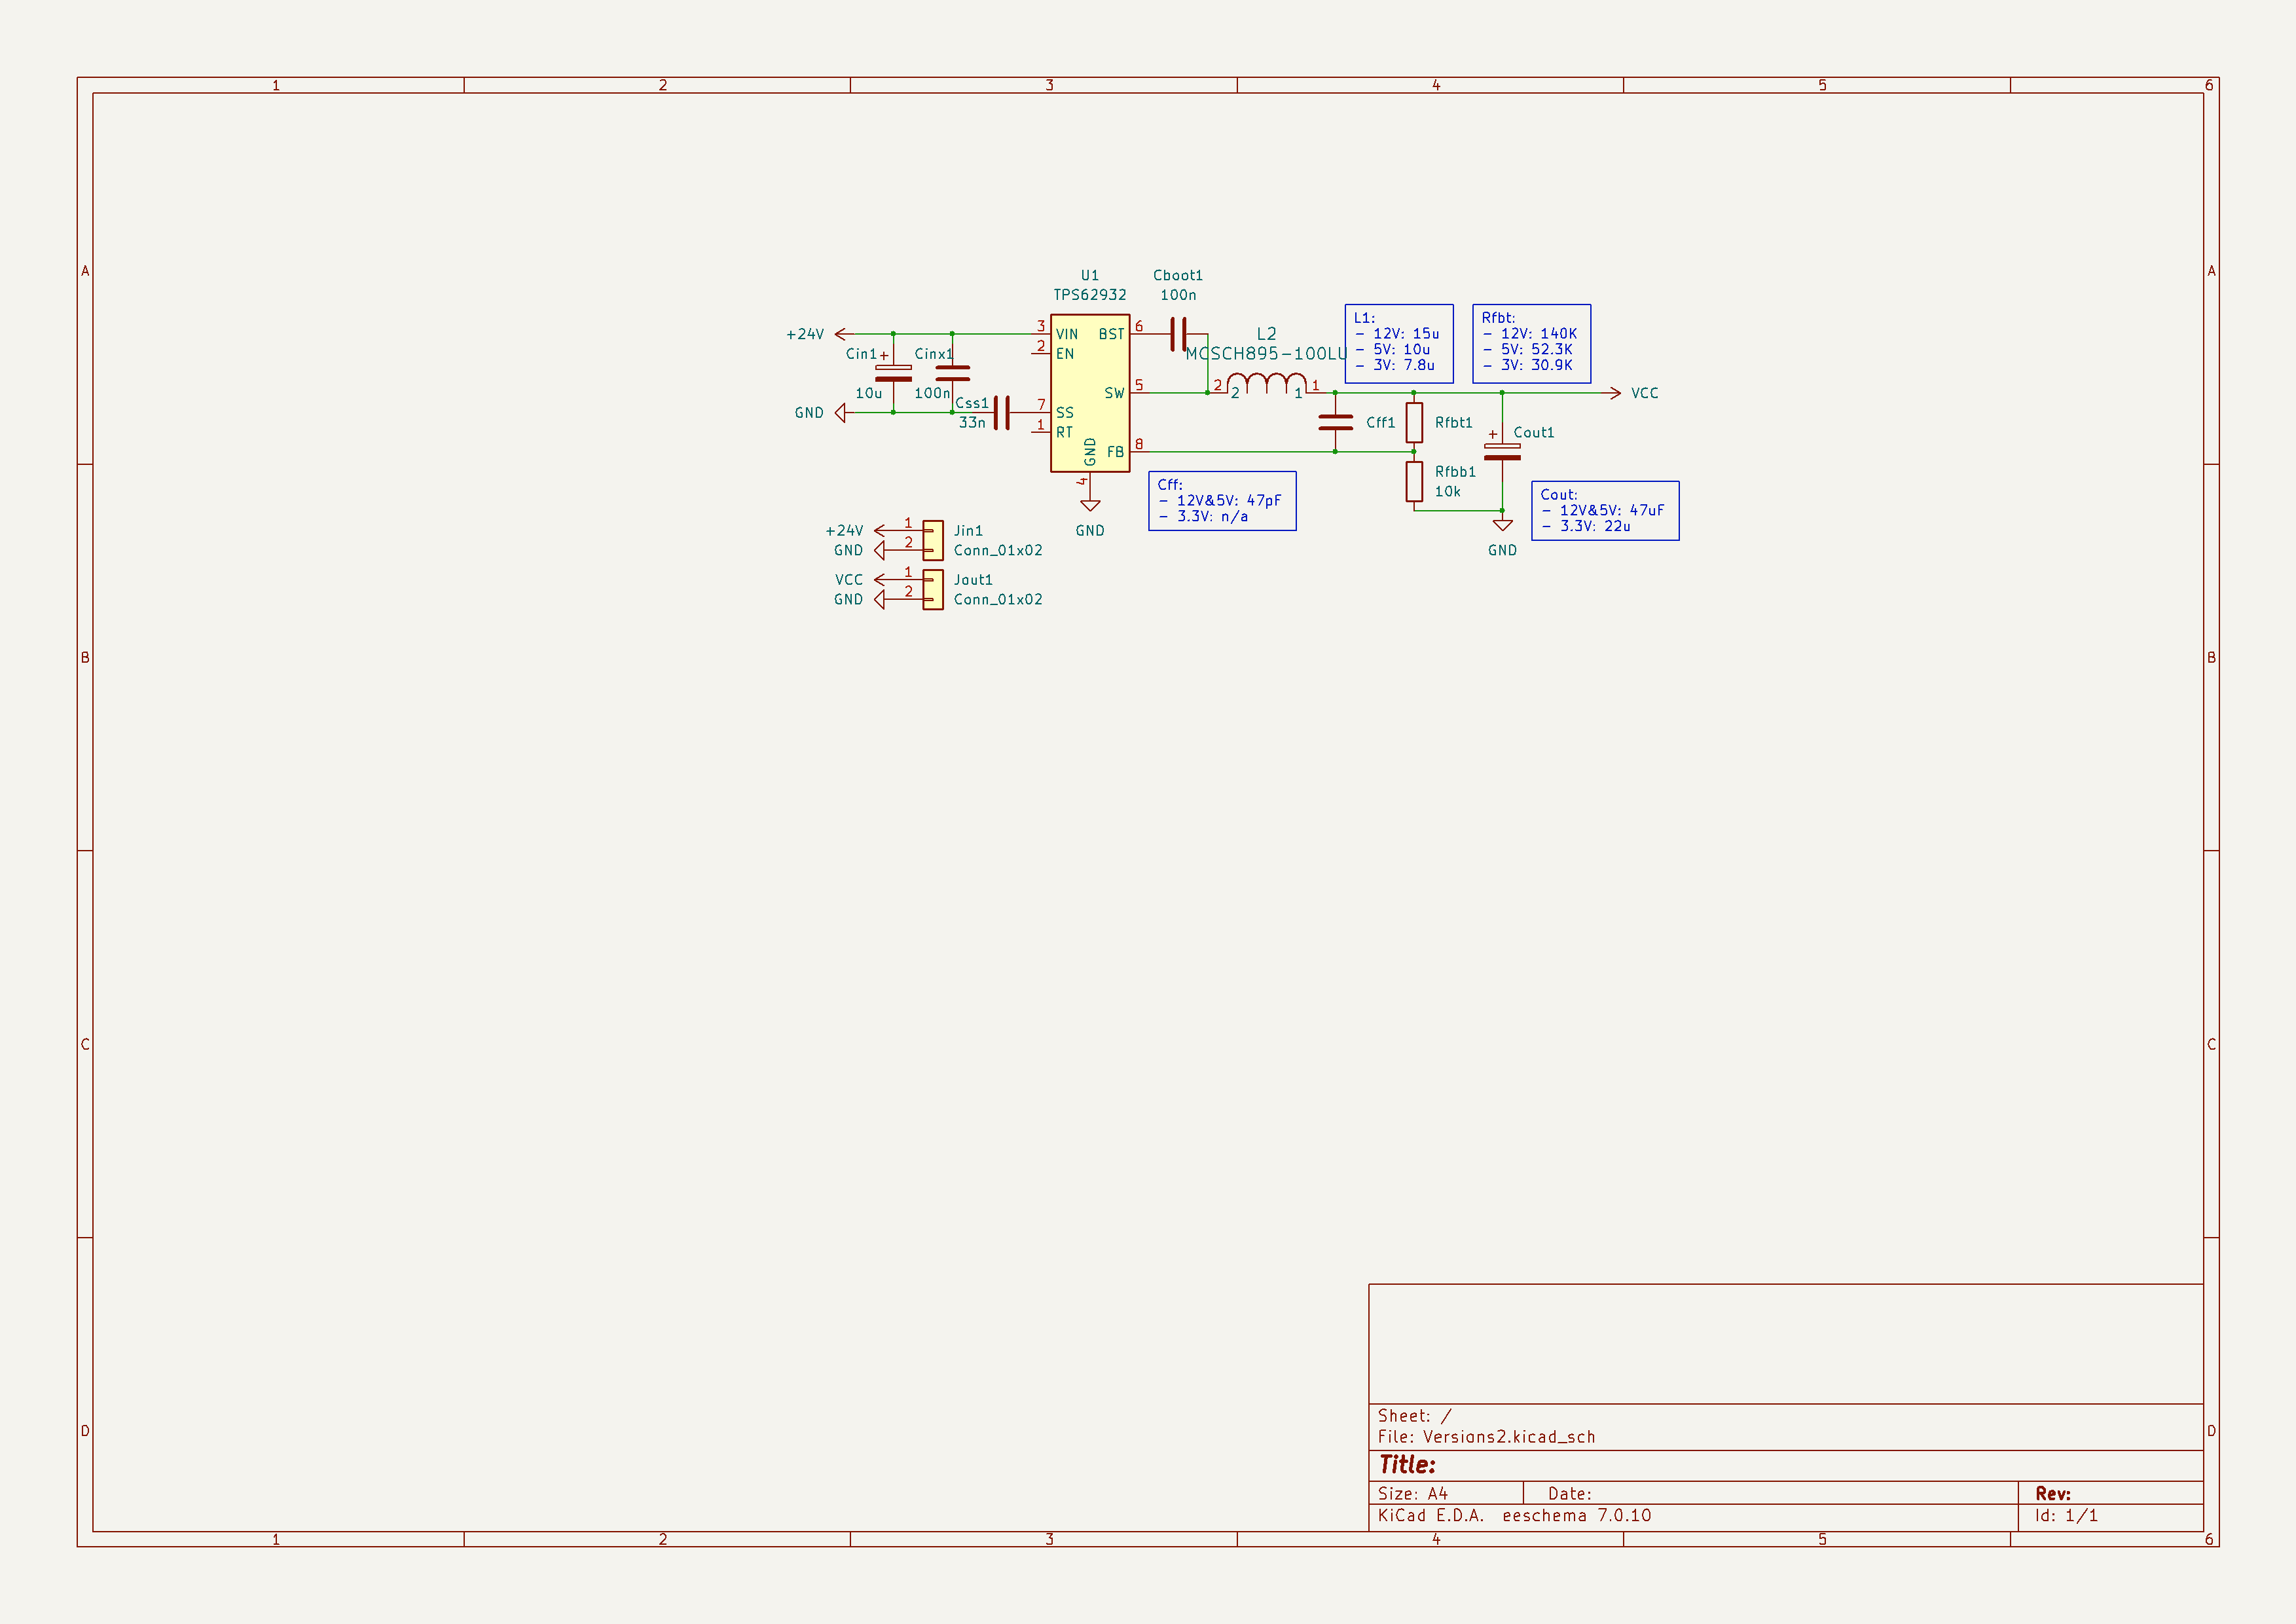
\includegraphics[trim=1150 1500 900 350,clip,width=0.8\linewidth]{img//buckconverters/circuit.png}
    \caption{Circuit: Versatile Buck converter}
    \label{fig:circuit_buck_converter}
\end{figure}
For testing purposes, a versatile circuit has been designed, allowing the generation of various voltages by making minor component changes, as depicted in \autoref{fig:circuit_buck_converter}. The decision to use a buck converter aligns with industry standards for dropping voltages efficiently. This approach ensures that the electric bike motor operates with high efficiency, a critical factor in achieving optimal performance and energy utilization in the context of an electrical bike motor.

\subsection{24V to 12V}
\subsubsection{Gate Driver Requirements}
Gate drivers play a crucial role in power electronics, facilitating the control of high-power semiconductor devices such as MOSFETs and IGBTs. In our system, the gate drivers are specified to operate within a voltage range of 10V to 20V. To meet this requirement, a 24V to 12V buck converter is employed to provide a stable and regulated 12V supply.

\autoref{section:gatedriver} provides additional details about the gate driver specifications.

\autoref{fig:buckconverter12v_VINVOUT} illustrates the voltage relationship between the input (24V) and output (12V) of the buck converter.
\begin{figure}[H]
    \centering
    \includegraphics[trim=0 235 0 70,clip,width=0.8\linewidth,page=8]{img//buckconverters//12v/WBDesign3.pdf}
    \caption{Buck converter 12V: Voltage in, Voltage out from: %\autoref{appendix:buckconverter}
    }
    \label{fig:buckconverter12v_VINVOUT}
\end{figure}

\subsubsection{Performance Analysis}
To ensure the reliability and stability of the 24V to 12V buck converter in our design, a series of simulations have been conducted. The following sections provide a detailed analysis of key performance aspects.

\subsubsection{Bode Plot Analysis}
The frequency response of the buck converter is analyzed through a Bode plot, as depicted in \autoref{fig:buckconverter12v_bodeplot}. This analysis provides insights into the converter's gain and phase margins, allowing us to assess its stability and transient response.
\begin{figure}[H]
    \centering
    \includegraphics[trim=0 165 0 70,clip,width=0.8\linewidth,page=8]{img//buckconverters//12v/WBDesign3_Bode Plot.pdf}
    \caption{Buck converter 12V: Bode plot Simulation from: %\autoref{appendix:buckconverter12v_bodeplot_full}
    }
    \label{fig:buckconverter12v_bodeplot}
\end{figure}

\subsubsection{Input Transient Simulation}
\autoref{fig:buckconverter12v_inputtransient} illustrates the response of the buck converter to input voltage transients. This simulation is crucial to evaluate the converter's ability to handle sudden changes in the input voltage and maintain stability during dynamic conditions.
\begin{figure}[H]
    \centering
    \includegraphics[trim=0 205 0 70,clip,width=0.8\linewidth,page=8]{img//buckconverters//12v/WBDesign3_Input Transient.pdf}
    \caption{Buck converter 12V: Input transient Simulation from: %\autoref{appendix:buckconverter12v_inputtransient_full}
    }
    \label{fig:buckconverter12v_inputtransient}
\end{figure}

\subsubsection{Load Transient Simulation}
The load transient simulation, shown in \autoref{fig:buckconverter12v_loadtransient}, assesses the converter's response to sudden changes in the output load. This is critical for ensuring that the converter can adapt and maintain a stable output voltage under varying load conditions.
\begin{figure}[H]
    \centering
    \includegraphics[trim=0 235 0 70,clip,width=0.8\linewidth,page=8]{img//buckconverters//12v/WBDesign3_Load Transient.pdf}
    \caption{Buck converter 12V: Load transient Simulation from: %\autoref{appendix:buckconverter12v_loadtransient_full}
    }
    \label{fig:buckconverter12v_loadtransient}
\end{figure}

\subsubsection{Startup Simulation}
The startup simulation, presented in \autoref{fig:buckconverter12v_startup}, examines the behavior of the buck converter during the initial power-up phase. It assesses the startup time and the stability of the output voltage during this crucial period.
\begin{figure}[H]
    \centering
    \includegraphics[trim=0 235 0 70,clip,width=0.8\linewidth,page=8]{img//buckconverters//12v/WBDesign3_Startup.pdf}
    \caption{Buck converter 12V: Startup Simulation from: %\autoref{appendix:buckconverter12v_startup_full}
    }
    \label{fig:buckconverter12v_startup}
\end{figure}

\subsubsection{Steady State Simulation}
\autoref{fig:buckconverter12v_SteadyState} illustrates the steady-state performance of the buck converter. This simulation confirms the converter's ability to provide a stable 12V output voltage under continuous operation.
\begin{figure}[H]
    \centering
    \includegraphics[trim=0 200 0 70,clip,width=0.8\linewidth,page=8]{img//buckconverters//12v/WBDesign3_Steady State.pdf}
    \caption{Buck converter 12V: Steady State Simulation from: %\autoref{appendix:buckconverter12v_SteadyState_full}
    }
    \label{fig:buckconverter12v_SteadyState}
\end{figure}

\subsubsection{Conclusion}
The 24V to 12V buck converter has been successfully designed to meet the power supply requirements of the gate drivers, operating in the specified range of 10V to 20V. Through comprehensive simulations, including Bode plot analysis, input and load transient simulations, startup, and steady-state simulations, the converter's performance has been thoroughly evaluated. The results demonstrate the converter's stability, reliability, and ability to maintain a constant output voltage under various operating conditions, ensuring optimal functionality of the gate drivers in our system.


\subsection{24V to 5V}
In the design and implementation of electronic systems, the need often arises to convert voltage levels to match the requirements of various components. This report addresses the specific task of converting a 24V input voltage to a 5V output voltage using a buck converter. The motivation behind this conversion is to provide a common voltage supply for components such as the hall sensor \autoref{section:hallsensor} (5V-20V), Raspberry Pi \autoref{section:interface} (5V), and touchscreen \autoref{section:interface}  (5V). The choice of 5V aligns with industry-standard operating voltages.

\subsubsection{Component Voltage Requirements}
The hall sensor, Raspberry Pi, and touchscreen in our system all operate at a common voltage of 5V. To ensure proper functionality and compatibility, a 24V to 5V buck converter is employed to provide a stable and regulated 5V supply.

\autoref{section:hallsensor}, \autoref{section:interface}, and \autoref{section:STM32F411CEU6} provide additional details about the specific components in the system.

\autoref{fig:buckconverter5v_VINVOUT} illustrates the relationship between the input (24V) and output (5V) voltages of the buck converter.
\begin{figure}[H]
    \centering
    \includegraphics[trim=0 235 0 70,clip,width=0.8\linewidth,page=3]{img//buckconverters//5v/WBDesign2.pdf}
    \caption{Buck converter 5V: Voltage in, Voltage out from: %\autoref{appendix:buckconverter5v_VINVOUT_full}
    }
    \label{fig:buckconverter5v_VINVOUT}
\end{figure}

\subsubsection{Performance Analysis}
To ensure the reliability and stability of the buck converter in our design, a series of simulations have been conducted. The following sections provide a detailed analysis of key performance aspects.

\subsubsection{Bode Plot Analysis}
The frequency response of the buck converter is examined through a Bode plot analysis, as depicted in \autoref{fig:buckconverter5v_bodeplot}. This analysis provides insights into the converter's gain and phase margins, allowing us to assess its stability and transient response.
\begin{figure}[H]
    \centering
    \includegraphics[trim=0 165 0 70,clip,width=0.8\linewidth,page=8]{img//buckconverters//5v/WBDesign2_Bode Plot.pdf}
    \caption{Buck converter 5V: Bode plot Simulation from: %\autoref{appendix:buckconverter5v_bodeplot_full}
    }
    \label{fig:buckconverter5v_bodeplot}
\end{figure}

\subsubsection{Input Transient Simulation}
\autoref{fig:buckconverter5v_inputtransient} illustrates the response of the buck converter to input voltage transients. This simulation is crucial to evaluate the converter's ability to handle sudden changes in the input voltage and maintain stability during dynamic conditions.
\begin{figure}[H]
    \centering
    \includegraphics[trim=0 205 0 70,clip,width=0.8\linewidth,page=8]{img//buckconverters//5v/WBDesign2_Input Transient.pdf}
    \caption{Buck converter 5V: Input transient Simulation from: %\autoref{appendix:buckconverter5v_inputtransient_full}
    }
    \label{fig:buckconverter5v_inputtransient}
\end{figure}

\subsubsection{Load Transient Simulation}
The load transient simulation, shown in \autoref{fig:buckconverter5v_loadtransient}, assesses the converter's response to sudden changes in the output load. This is critical for ensuring that the converter can adapt and maintain a stable output voltage under varying load conditions.
\begin{figure}[H]
    \centering
    \includegraphics[trim=0 235 0 70,clip,width=0.8\linewidth,page=8]{img//buckconverters//5v/WBDesign2_Load Transient.pdf}
    \caption{Buck converter 5V: Load transient Simulation from: %\autoref{appendix:buckconverter5v_loadtransient_full}
    }
    \label{fig:buckconverter5v_loadtransient}
\end{figure}

\subsubsection{Startup Simulation}
The startup simulation, presented in \autoref{fig:buckconverter5v_startup}, examines the behavior of the buck converter during the initial power-up phase. It assesses the startup time and the stability of the output voltage during this crucial period.
\begin{figure}[H]
    \centering
    \includegraphics[trim=0 235 0 70,clip,width=0.8\linewidth,page=8]{img//buckconverters//5v/WBDesign2_Startup.pdf}
    \caption{Buck converter 5V: Startup Simulation from: %\autoref{appendix:buckconverter5v_startup_full}
    }
    \label{fig:buckconverter5v_startup}
\end{figure}

\subsubsection{Steady State Simulation}
\autoref{fig:buckconverter5v_SteadyState} illustrates the steady-state performance of the buck converter. This simulation confirms the converter's ability to provide a stable 5V output voltage under continuous operation.
\begin{figure}[H]
    \centering
    \includegraphics[trim=0 200 0 70,clip,width=0.8\linewidth,page=8]{img//buckconverters//5v/WBDesign2_Steady State.pdf}
    \caption{Buck converter 5V: Steady State Simulation from: %\autoref{appendix:buckconverter5v_SteadyState_full}
    }
    \label{fig:buckconverter5v_SteadyState}
\end{figure}

\subsubsection{Conclusion}
The 24V to 5V buck converter has been successfully designed to meet the power supply requirements of the hall sensor, Raspberry Pi, and touchscreen, all operating at a common voltage of 5V. Through comprehensive simulations, including Bode plot analysis, input and load transient simulations, startup, and steady-state simulations, the converter's performance has been thoroughly evaluated. The results demonstrate the converter's stability, reliability, and ability to maintain a constant output voltage under various operating conditions, ensuring optimal functionality of the components in our system.


% \subsection{24V to 3.3V}
% In the design and operation of electronic systems, it is often necessary to convert voltage levels to match the requirements of specific components. In our case, the input voltage to an STM32 microcontroller is 3.3V, while the available power source provides 24V. This necessitates the use of a voltage regulator to step down the voltage from 24V to 3.3V. The chosen solution for this task is a buck converter.

% \subsubsection{STM32 Microcontroller Requirements}
% The STM32 microcontroller used in our application, specifically the STM32F411CEU6 model, requires a stable power supply of 3.3V. To meet this requirement, we employ a buck converter to step down the 24V input voltage to the desired 3.3V output voltage.

% \autoref{fig:buckconverter3v3_VINVOUT} illustrates the voltage relationship between the input (24V) and output (3.3V) of the buck converter.
% \begin{figure}[H]
%     \centering
%     \includegraphics[trim=0 235 0 70,clip,width=0.8\linewidth,page=7]{img//buckconverters//3v3/WBDesign4.pdf}
%     \caption{Buck converter 3.3V: Voltage in, Voltage out from: %\autoref{appendix:buckconverter3v3_VINVOUT_full}
%     }
%     \label{fig:buckconverter3v3_VINVOUT}
% \end{figure}

% \subsubsection{Buck Converter Performance Analysis}
% To ensure the reliability and stability of the buck converter in our design, various simulations have been conducted. The following sections provide an in-depth analysis of the key aspects of the buck converter's performance.


% \subsubsection{Bode Plot Analysis}
% The frequency response of the buck converter is crucial for understanding its stability and transient response. The Bode plot, shown in \autoref{fig:buckconverter3v3_bodeplot}, provides insights into the converter's gain and phase margins, allowing us to assess its stability under different operating conditions.
% \begin{figure}[H]
%     \centering
%     \includegraphics[trim=0 165 0 70,clip,width=0.8\linewidth,page=7]{img//buckconverters//3v3/WBDesign4_Bode Plot-5.pdf}
%     \caption{Buck converter 3.3V: Bode plot Simulation from: %\autoref{appendix:buckconverter3v3_bodeplot_full}
%     }
%     \label{fig:buckconverter3v3_bodeplot}
% \end{figure}

% \subsubsection{Input Transient Simulation}
% \autoref{fig:buckconverter3v3_inputtransient} depicts the response of the buck converter to input voltage transients. This simulation helps evaluate how well the converter handles sudden changes in the input voltage, ensuring stability during dynamic conditions.
% \begin{figure}[H]
%     \centering
%     \includegraphics[trim=0 205 0 70,clip,width=0.8\linewidth,page=7]{img//buckconverters//3v3/WBDesign4_Input Transient-3.pdf}
%     \caption{Buck converter 3.3V: Input transient Simulation from: %\autoref{appendix:buckconverter3v3_inputtransient_full}
%     }
%     \label{fig:buckconverter3v3_inputtransient}
% \end{figure}

% \subsubsection{Load Transient Simulation}
% In \autoref{fig:buckconverter3v3_loadtransient}, the load transient simulation illustrates the converter's response to sudden changes in the output load. This is a critical aspect of performance, ensuring the converter can adapt and maintain stable output voltage under varying load conditions.
% \begin{figure}[H]
%     \centering
%     \includegraphics[trim=0 235 0 70,clip,width=0.8\linewidth,page=5]{img//buckconverters//3v3/WBDesign4_Load Transient-2.pdf}
%     \caption{Buck converter 3.3V: Load transient Simulation from: %\autoref{appendix:buckconverter3v3_loadtransient_full}
%     }
%     \label{fig:buckconverter3v3_loadtransient}
% \end{figure}

% \subsubsection{Startup Simulation}
% The startup simulation, as shown in \autoref{fig:buckconverter3v3_startup}, examines the behavior of the buck converter during the initial power-up phase. It assesses the startup time and the stability of the output voltage during this critical period.
% \begin{figure}[H]
%     \centering
%     \includegraphics[trim=0 235 0 70,clip,width=0.8\linewidth,page=7]{img//buckconverters//3v3/WBDesign4_Startup-1.pdf}
%     \caption{Buck converter 3.3V: Startup Simulation from: %\autoref{appendix:buckconverter3v3_startup_full}
%     }
%     \label{fig:buckconverter3v3_startup}
% \end{figure}

% \subsubsection{Steady State Simulation}
% \autoref{fig:buckconverter3v3_SteadyState} illustrates the steady-state performance of the buck converter, confirming its ability to provide a stable 3.3V output voltage under continuous operation.
% \begin{figure}[H]
%     \centering
%     \includegraphics[trim=0 200 0 70,clip,width=0.8\linewidth,page=7]{img//buckconverters//3v3/WBDesign4_Steady State-4.pdf}
%     \caption{Buck converter 3.3V: Steady State Simulation from: %\autoref{appendix:buckconverter3v3_SteadyState_full}
%     }
%     \label{fig:buckconverter3v3_SteadyState}
% \end{figure}

% \subsubsection{Conclusion}
% The 24V to 3.3V buck converter has been successfully designed to meet the power supply requirements of the STM32 microcontroller. Through comprehensive simulations, including Bode plot analysis, input and load transient simulations, startup, and steady-state simulations, the converter's performance has been thoroughly evaluated. The results demonstrate the converter's stability, reliability, and ability to maintain a constant output voltage under various operating conditions, ensuring optimal functionality of the STM32 microcontroller in our application.